\documentclass{uimppracticas}

%Permitir cabeceras y pie de páginas personalizados
\pagestyle{fancy}

%Path por defecto de las imágenes
\graphicspath{ {./images/} }

%Declarar formato de encabezado y pie de página de las páginas del documento
\fancypagestyle{doc}{
%Pie de Página
\footerpr{}{}{{\thepage} de \pageref{LastPage}}
}

%Declarar formato de encabezado y pie del título e indice
\fancypagestyle{titu}{%
%Cabecera
\headerpr{}{}{}
%Pie de Página
\footerpr{}{}{}
}

\appto\frontmatter{\pagestyle{titu}}
\appto\mainmatter{\pagestyle{doc}}

\begin{document}

%Comienzo formato título
\frontmatter

%Portada (Centrado todo)
\centeredtitle{./images/LogoUIMP.png}{Máster Universitario en Investigación en Inteligencia Artificial}{Curso 2020-2021}{Recuperación y extracción de información, \\ grafos y redes sociales}{Práctica Bloque II: Recuperación de información y minería de texto}

\begin{center}
	\large \today
\end{center}

\vspace{40mm}

\begin{flushright}
	{\bf Laura Rodríguez Navas}\\
	\textbf{DNI:} 43630508Z\\
	\textbf{e-mail:} \href{rodrigueznavas@posgrado.uimp.es}{rodrigueznavas@posgrado.uimp.es}
\end{flushright}

\newpage

%Índice
\tableofcontents

\newpage

%Comienzo formato documento general
\mainmatter

\setlength\parskip{2.5ex}

\section{Resumen}

En esta práctica se ha implementado un rastreador web (crawler) en Python (ver Sección~\ref{crawler}), que se complementa con un proceso de agrupamiento (ver Sección~\ref{kmeans}), también implementado en Python, de la información extraída por el rastreador web. En este documento se describe el desarrollo paso a paso, que se puede descargar de~\cite{GitHubRepo}.

\section{Rastreador web}\label{crawler}

En esta sección se describe como se ha implementado el rastreador web (crawler) en Python usando la librería \href{https://scrapy.org/}{Scrapy}, y para empezar este desarrollo se ejecutó el siguiente comando:

\begin{lstlisting}[language=bash, basicstyle=\small]
$ scrapy startproject books
\end{lstlisting}

Este comando crea un proyecto Scrapy en el directorio books, siguiendo la \href{https://docs.scrapy.org/en/latest/topics/commands.html#default-structure-of-scrapy-projects}{estructura por defecto} común para todo proyecto Scrapy. El comando también crea el fichero \textit{scrapy.cfg}, que contiene el nombre del módulo en Python que define la configuración del proyecto books. El proyecto Scrapy de la práctica lo he llamado books, porqué se rastrea y recupera información de un catálogo de libros, que podemos encontrar en el siguiente enlace a la página web: \url{http://books.toscrape.com}.

Una vez se ha creado el proyecto con el comando anterior, se deben que definir los ítems de cada libro que se quieran extraer del catálogo web. En este caso los ítems que se extraen son: el título, la categoría, la descripción, el precio y la valoración de cada libro. Para que el rastreador lo tenga en cuenta, se tiene que modificar el fichero \textit{books/items.py}, para incluir los cinco ítems que se quieren extraer. A continuación, podemos ver los ítems añadidos en el fichero \textit{items.py}:

\begin{lstlisting}[language=python, basicstyle=\small]
class BooksItem(scrapy.Item):
	# define the fields for your item here like:
	# name = scrapy.Field()
	title = scrapy.Field()
	category = scrapy.Field()
	description = scrapy.Field()
	price = scrapy.Field()
	rating = scrapy.Field()
\end{lstlisting}

El siguiente paso es describir la manera de extraer la información de estos ítems. Para ello, se utilizan reglas de expresión \href{https://www.w3.org/TR/xpath/all/}{XPath} y \href{https://www.w3.org/TR/selectors/}{CSS}. Por ejemplo, si nos fijamos en el código HTML de uno de los libros que se van rastrear (ver Figura \ref{book}), veremos que el título del libro es fácil de extraer con la siguiente regla de expresión CSS: \textbf{"h1 ::text"}. Por otro lado, cuando la extracción de información se complica un poco más, se usan reglas de expresión XPath. Por ejemplo, para extraer las descripciones de todos los libros se usa la regla de expresión: \textbf{"//div[@id='product\_description']/following-sibling::p/text()"}. 

En este documento no se describen todas las reglas de expresión que se han desarrollado, pero se pueden consultar en~\cite{GitHubRepo}, concretamente en el fichero \textit{books/spiders/books\_toscrape.py}. Este fichero es la araña o más comúnmente llamada en inglés \textit{spider}, que contiene todas las reglas de expresión de cada uno de los ítems de \textit{items.py}, para definir cómo se va a rastrear y cómo se va a extraer la información del catálogo de libros en la web.

\begin{figure}[h]
	\centering
	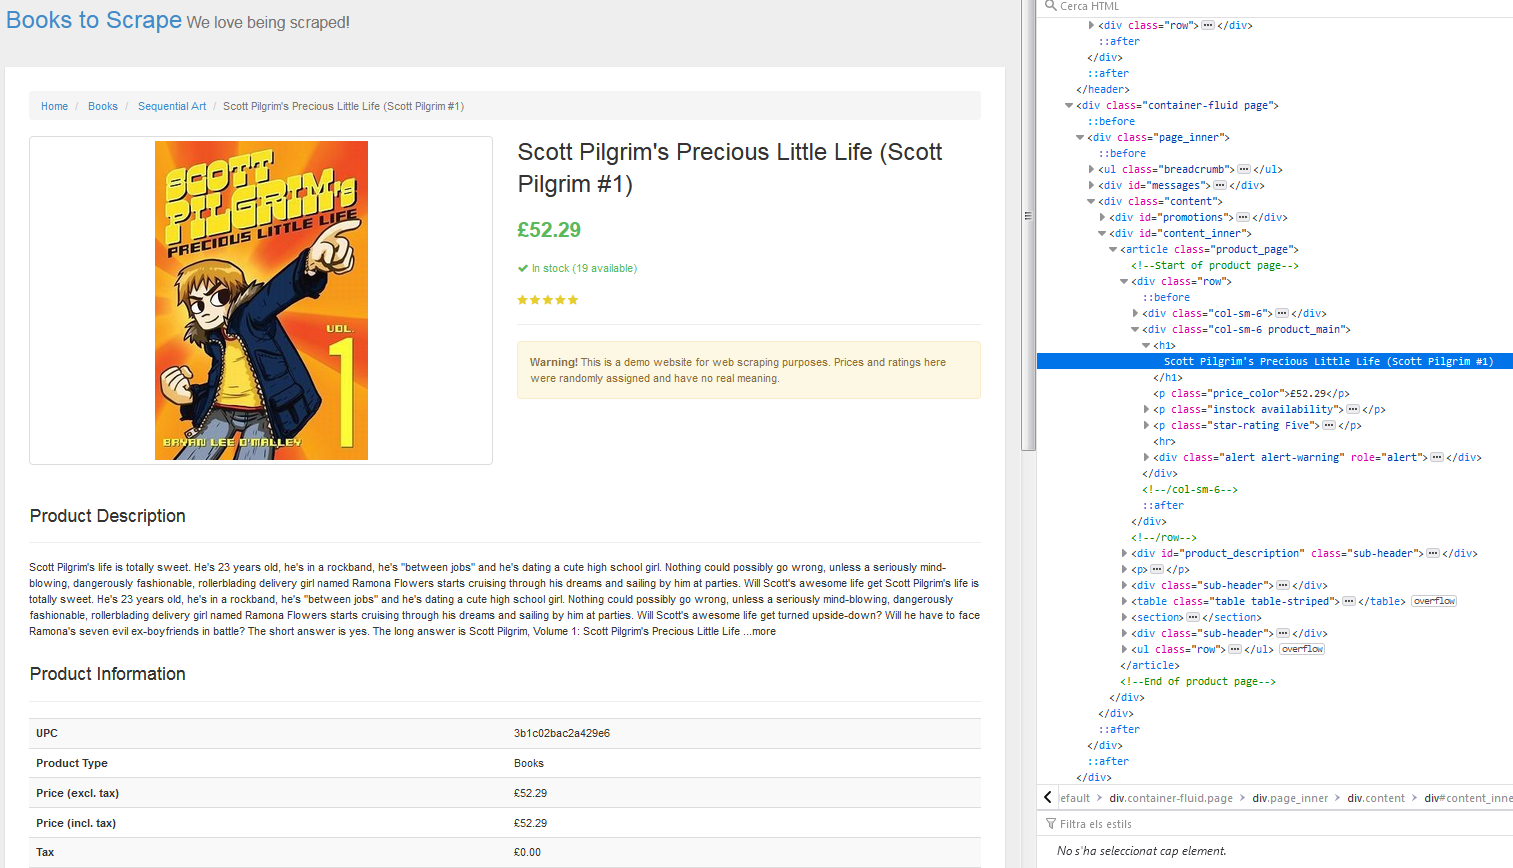
\includegraphics[scale=0.37]{images/book}
	\caption{Ejemplo de libro a rastrear.}
	\label{book}
\end{figure}

\begin{definition}\label{spider}
	Las arañas son clases en Python que definen cómo se rastrea una página web determinada (o un grupo de páginas web), incluido cómo realizar el rastreo y cómo extraer la información deseada. En otras palabras, las arañas son el lugar donde se define el comportamiento personalizado para rastrear y analizar las páginas web.
\end{definition}

En las arañas también se tienen que especificar las solicitudes iniciales de todas las URLs a rastrear y crear una función de devolución de llamada (\textit{parse}), a la que se llamará para generar los ítems de respuesta de esas solicitudes. Por último, la información devuelta por las arañas, normalmente se conserva en una base de datos o se escribe en un archivo. En el caso de la práctica, la información de los ítems: título, categoría, descripción, precio y valoración de cada libro, que son devueltos por la araña \textit{books.toscrape}, se guardan en el archivo \textit{books.json}. 

La araña desarrollada en esta práctica (\textit{books.toscrape}), que procesa todas las URLs descubiertas de \url{http://books.toscrape.com}, utilizando la función \textit{parse}, que a su vez llama a la función \textit{parse\_book\_page} donde se definen todas las reglas de expresión, se muestra a continuación:

\begin{lstlisting}[language=python, basicstyle=\small]
class BooksToscrapeSpider(scrapy.Spider):
	name = 'books.toscrape'
	allowed_domains = ['books.toscrape.com']
	start_urls = ['http://books.toscrape.com/']
	
	def parse(self, response):
		for book_url in response.css("article.product_pod > h3 > a ::attr(href)").extract():
			yield scrapy.Request(response.urljoin(book_url), callback=self.parse_book_page)
		next_page = response.css("li.next > a ::attr(href)").extract_first()
		if next_page:
			yield scrapy.Request(response.urljoin(next_page), callback=self.parse)
	
	@staticmethod
	def parse_book_page(response):
		item = {}
		product = response.css("div.product_main")
		item["title"] = product.css("h1 ::text").extract_first()
		item['category'] = response.xpath("//ul[@class='breadcrumb']/li[@class='active']/preceding-sibling::li[1]/a/text()").extract_first()
		item['description'] = response.xpath("//div[@id='product_description']/following-sibling::p/text()").extract_first()
		price = response.xpath('//th[text()="Price (incl. tax)"]/following-sibling::td/text()').extract_first()
		item['price'] = price.replace('£', '')
		rating = response.xpath('//*[contains(@class, "star-rating")]/@class').extract_first()
		item['rating'] = rating.replace('star-rating ', '')
		yield item
\end{lstlisting}

A partir de este momento, ya podemos iniciar la araña para que recupere la información de los libros del catálogo web y la escriba en el archivo \textit{books.json}, aunque primero es recomendable modificar el fichero \textit{books/settings.py}, para limitar el acceso de la araña, ya que podemos generar un ataque \href{https://es.wikipedia.org/wiki/Ataque\_de\_denegaci\%C3\%B3n_de_servicio}{DDoS}. Para no provocar un ataque de este tipo, debemos descomentar la variable \href{https://docs.scrapy.org/en/latest/topics/settings.html#download-delay}{DOWNLOAD\_DELAY} del fichero \textit{books/settings.py}  y darle un valor en segundos (p.ej. DOWNLOAD\_DELAY = 3). 

Finalmente, para iniciar la araña se deben ejecutar los comandos siguientes:	

\begin{lstlisting}[language=bash, basicstyle=\small]
$ cd books
$ scrapy crawl books.toscrape -o books.json
\end{lstlisting}

\section{K-Means}\label{kmeans} 

En esta sección se describe como se ha desarrollado el proceso de agrupamiento en Python, de los datos recuperados por el rastreador web (crawler) usando la librería scikit-learn~\cite{scikit-learn}. El código llevado a cabo se encuentra en el directorio kmeans de~\cite{GitHubRepo}, que contiene el algoritmo de agrupación elegido para esta práctica:  \href{https://scikit-learn.org/stable/modules/generated/sklearn.cluster.KMeans.html}{el algoritmo K-Means}. K-Means es un algoritmo no supervisado de clustering, que usualmente se utiliza cuando tenemos un montón de datos sin etiquetar, con el objetivo de encontrar "K" grupos o clústeres entre el conjunto de datos. En el caso de la práctica, el algoritmo K-Means agrupará los títulos de los libros del catálogo web en diferentes clústeres, y en este caso, el tipo de agrupamiento se denomina \href{https://en.wikipedia.org/wiki/Document_clustering}{\textit{clustering}} de textos.

\subsection{Datos de entrada}

En esta sección se concreta el conjunto de datos que utilizaremos para alimentar el algoritmo K-Means. Para ello, primero se empieza extrayendo la información de los libros almacenada en el fichero \textit{books/books.json}. Segundo, convertimos esta información en un \textit{DataFrame} (ver Definición~\ref{dataframe}). Además, eliminamos los valores no válidos que pudieran existir en el \textit{DataFrame} y finalmente, este es almacenado en un fichero CSV (\textit{kmeans/books.csv}). Para este procedimiento se ha usado la librería pandas~\cite{jeff_reback_2020_4309786}. A continuación, podemos observar las primeras líneas del contenido del \textit{DataFrame} que forman los datos de entrada:

\begin{table}[h]
	\begin{adjustbox}{width=\columnwidth,center}
		\begin{tabular}{lllll}
			\toprule
			title & category & description & price & rating \\
			\midrule
			Sapiens: A Brief History of Humankind & History & From a renowned historian... & 54.23 & Five \\
			Sharp Objects & Mystery & WICKED above her hipbone, GIRL... & 47.82 & Four \\
			Soumission & Fiction & Dans une France assez... & 50.10 & One \\
			Tipping the Velvet & Historical Fiction & Erotic and absorbing... & 53.74 & One \\
			A Light in the Attic & Poetry & It's hard to imagine... & 51.77 & Three \\
			\bottomrule
		\end{tabular}
	\end{adjustbox}
	\caption{Conjunto de datos de entrada.}
	\label{table1}
\end{table}

Concretamente, la estructura de datos que se utilizará para alimentar el algoritmo K-Means, está formada por la siguiente lista que contiene los títulos de los libros. Vemos los diez primeros:

\begin{lstlisting}[language=python, basicstyle=\small]
titles = df["title"].to_list()
print(titles[:10])  # first 10 titles
>> ['Sapiens: A Brief History of Humankind', 'Sharp Objects', 'Soumission', 'Tipping the Velvet', 'A Light in the Attic', "It's Only the Himalayas", 'Libertarianism for Beginners', 'Mesaerion: The Best Science Fiction Stories 1800-1849', 'Olio', 'Our Band Could Be Your Life: Scenes from the American Indie Underground, 1981-1991']
\end{lstlisting}

\begin{definition}\label{dataframe}
	Un DataFrame es una estructura de datos etiquetada bidimensional que acepta diferentes tipos datos de entrada organizados en columnas. Se puede pensar en un DataFrame como una hoja de cálculo o una tabla SQL.
\end{definition}

\subsection{Palabras vacías, segmentación y tokenización}\label{stem_token}

Esta sección se centra en describir algunas funciones para transformar el conjunto de datos de entrada y así facilitar la ejecución del algoritmo K-Means. Porqué siempre es una buena idea indexar el conjunto de datos, en este caso de textos, a la hora de realizar un procedimiento de agrupamiento. Hay, por supuesto, muchos tipos de indexaciones, y a continuación se describe la transformación del conjunto de datos que se usa en esta práctica.

Para poder realizar un proceso de indexación de los títulos, se obtienen la lista de palabras vacías en inglés (ver Definición~\ref{palabras_vacías}), y el \href{https://www.nltk.org/_modules/nltk/stem/snowball.html}{Snowball Stemmer} con la ayuda de la librería NLTK~\cite{bird2009natural}. Tanto para la lista de las palabras vacías (\textit{stopwords}) o para el Snowball Stemmer se indica el idioma: inglés; ya que los títulos de los libros están inglés. 

\begin{lstlisting}[language=python, basicstyle=\small]
# nltk's English stopwords as variable called 'stopwords'	
stopwords = nltk.corpus.stopwords.words('english')  
# nltk's SnowballStemmer as variabled 'stemmer'
stemmer = SnowballStemmer("english")
print(stopwords[:10])   # first 10 stopwords
>> ['i', 'me', 'my', 'myself', 'we', 'our', 'ours', 'ourselves', 'you', "you're"]    
\end{lstlisting}

\begin{definition}\label{palabras_vacías}
	Las palabras vacías son palabras sin significado como artículos, pronombres, preposiciones, etc. que son filtradas antes o después del procesamiento de datos en lenguaje natural (texto). Por ejemplo: "a", "the", o "in" que no transmiten un significado significativo.
\end{definition}

La obtención de estos dos elementos es necesaria para realizar los procesos de indexación: tokenización y segmentación (stemming) sobre los títulos. Concretamente, el proceso de tokenización divide las cadenas de texto más largas de los títulos en cadenas más pequeñas o tokens. Y el proceso de segmentación extrae las raíces de los tokens. El proceso de segmentación se realiza porque las raíces de los tokens pueden aparecer repetidamente en diferentes los títulos.

A continuación, vemos las funciones \textit{tokenize\_and\_stem} y \textit{tokenize\_only} que se han desarrollado para el proceso de indexación de esta práctica: 

\begin{lstlisting}[language=python, basicstyle=\small]
def tokenize_and_stem(text):
	tokens = [word for sent in nltk.sent_tokenize(text) for word in nltk.word_tokenize(sent)]
	filtered_tokens = []
	for token in tokens:
		if re.search('[a-zA-Z]', token):
			filtered_tokens.append(token)
	stems = [stemmer.stem(t) for t in filtered_tokens]
	return stems

def tokenize_only(text):
	tokens = [word.lower() for sent in nltk.sent_tokenize(text) for word in nltk.word_tokenize(sent)]
	filtered_tokens = []
	for token in tokens:
		if re.search('[a-zA-Z]', token):
			filtered_tokens.append(token)
	return filtered_tokens  
\end{lstlisting}

Estas funciones son casi iguales, ya que las dos realizan el mismo proceso de tokenización sobre un texto de entrada, pero no son exactamente iguales porqué la función \textit{tokenize\_and\_stem}, además, realiza un proceso de segmentación. Las funciones se usan para calcular la matriz tf-idf de la siguiente sección y para la visualización de los clústeres resultantes de la ejecución del algoritmo K-Means.

\subsection{Extracción de características}\label{características}

\begin{wrapfigure}[13]{r}{0.4\textwidth}
	\centering
	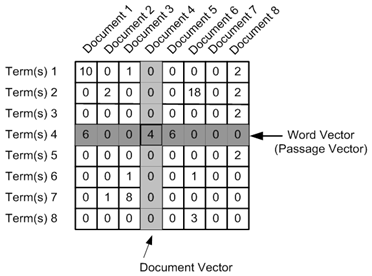
\includegraphics[width=0.4\textwidth]{images/matrix}
	\caption{Ejemplo de matriz tf-idf.}
	\label{matrix}
\end{wrapfigure}

En esta sección calcularemos la matriz \href{https://es.wikipedia.org/wiki/Tf-idf}{TF-IDF} (ver Figura~\ref{matrix}), porqué nos será muy útil para la agrupación de los títulos en clústeres, ya que nos ayudará a comprender qué tipo de títulos tenemos. El principal motivo para calcularla es por el proceso de agrupamiento en sí mismo. El clustering, como ya sabemos, es una técnica de aprendizaje automático no-supervisada. Esto implica que no es capaz de establecer la relación entre los conjuntos de datos de entrada y los resultados, sencillamente porque no hay resultados. Así que la responsabilidad de identificar qué atributos son relevantes recae sobre nosotros. 

El acrónimo TF-IDF significa en inglés \textit{Term Frequency-Inverse Document Frequency}, y representa una estadística numérica que demuestra la importancia de las palabras teniendo en cuenta los siguientes dos efectos:

\begin{itemize}
	\item Importancia del término en el documento (TF): un término que aparece muchas veces en un documento
	es más importante que otro que sólo aparece una vez.
	\begin{equation}
		\large TF_{ix} = \frac{n_{ix}}{max_{l} n_{l,x}}
	\end{equation}
	
	\item Importancia del término en la colección (IDF): un término que aparece pocas veces en la colección
	tiene un mayor poder discriminador que un término que aparece en todos los documentos.
	\begin{equation}
		\large IDF_i = log \frac{N}{n_{i}}
	\end{equation}
\end{itemize}

Donde $TD-IDF_{i,x}$ es igual al producto de $TF_{ix}$ con $IDF_{i}$.

\begin{equation}
	\large TD-IDF_{i,x} = TF_{ix} * IDF_{i}
\end{equation}

Para calcular los valores de la matriz TF-IDF por título se utiliza \href{https://scikit-learn.org/stable/modules/generated/sklearn.feature_extraction.text.TfidfVectorizer.html}{sklearn.feature\_extraction.text.TfidfVectorizer}, que una vez calculada, la podremos usar para alimentar el algoritmo K-Means. Pero antes, comentar un par de cosas a tener en cuenta sobre los parámetros definidos en la función \textit{TfidfVectorizer}:

\begin{itemize}
	\item use\_idf: habilitará la reponderación de frecuencia de documentos inversa.
	\item ngram\_range: define el límite inferior y superior del rango de n-valores para diferentes n-gramas que se extraerán. Ver Definición~\ref{n_grama}.
\end{itemize}

\begin{lstlisting}[language=python, basicstyle=\small]
tfidf_vectorizer = TfidfVectorizer(stop_words=stopwords, use_idf=True, tokenizer=tokenize_and_stem, ngram_range=(1, 3))

tfidf_matrix = tfidf_vectorizer.fit_transform(titles)
print(tfidf_matrix.shape)
>> (998, 7258)
\end{lstlisting}

Vemos que la matriz TD-IDF está formada por 998 términos y 7258 documentos. Es grande y seguramente tendremos problemas para mostrar visualmente los clústeres después de ejecutar K-Means.

\begin{definition}\label{n_grama}
	Un n-grama es una secuencia contigua de n elementos de una muestra determinada de texto o de un discurso. Los elementos pueden ser fonemas, sílabas, letras o palabras según la aplicación. Los n-gramas normalmente se recopilan de un texto.
\end{definition}

A continuación, mostramos que durante el proceso de creación de la matriz, la función \textit{TfidfVectorizer} ha creado un vocabulario de términos. Los primeros veinte términos del vocabulario son:

\begin{lstlisting}[language=python, basicstyle=\small]
terms = tfidf_vectorizer.get_feature_names()
print(terms[:20])    # first 20 terms
>> ["'d", "'d go", "'d go bernadett", "'m", "'m gone", "'m home", "'m lie", "'m lie tell", "'s", "'s alic", "'s alic wonderland", "'s astound", "'s astound stori", "'s autobiographi", "'s babi", "'s babi ice", "'s berlin", "'s call", "'s call cormoran", "'s childhood"]
\end{lstlisting}

\subsection{Entrenamiento del algoritmo}

Ahora pasamos a la parte divertida. Con la matriz TD-IDF calculada en la sección anterior, se puede ejecutar el algoritmo K-Means utilizando \href{https://scikit-learn.org/stable/modules/generated/sklearn.cluster.KMeans.html}{sklearn.cluster.KMeans}, para agrupar en diferentes clústeres los títulos por las palabras que contienen. Para ello, K-Means utiliza una proceso iterativo en el que se van ajustando los clústeres para producir el resultado final siguiendo los siguientes pasos:

\begin{itemize}
	\item Inicialización: se elige la localización de los centroides iniciales de los K clústeres aleatoriamente.
	\item Asignación: se asigna cada título al centroide más cercano.
	\item Actualización: se actualiza la posición del centroide a la media aritmética de las posiciones de los títulos asignados al clúster.
	\item Finalización: si el criterio de finalización se cumple, entonces se obtiene el resultado final. En caso contrario, ir se vuelve al paso 2 (Asignación).
\end{itemize}

A continuación, vemos como el algoritmo K-Means se ha implementado en Python, teniendo que indicar el número de clústeres que queremos encontrar.

\begin{lstlisting}[language=python, basicstyle=\small]
num_clusters = 40
kmeans = KMeans(n_clusters=num_clusters)
kmeans.fit(tfidf_matrix)
clusters = kmeans.labels_.tolist()
centroids = kmeans.cluster_centers_.argsort()[:, ::-1]
\end{lstlisting}

No es obvio, a priori, saber qué número de clústeres "K" es mejor. Por ejemplo, yo elegí 40, porqué el conjunto de datos de entrada contiene títulos que pertenecen al menos a una de las 50 categorías existentes del catálogo de libros, descartando 10 categorías que solo hacen referencia a un único libro. Pero para elegir el valor de "K", en general, no hay un modo exacto para determinar su valor, pero se puede estimar el valor con aceptable precisión siguiendo métodos más objetivos como: \href{https://en.wikipedia.org/wiki/Silhouette_(clustering)}{el método de la silueta} y \href{https://en.wikipedia.org/wiki/Elbow_method_(clustering)}{el método del codo}. Aunque en el caso de la práctica se ha probado el método del codo, pero al no devolver un valor aceptable se ha descartado.  

Así, como se comenta brevemente en la sección~\ref{características}, la preocupación de no poder representar gráficamente los resultados y visualizar los clústeres a causa del gran volumen de datos se cumple. No he encontrado una manera aceptable de visualizar los clústeres gráficamente y he optado por otra opción: mostrar los diez términos más frecuentes de cada clúster.

Para ello, primero crearemos dos nuevos dataframes. Uno que contenga los títulos y sus clústeres asignados (llamado \textit{frame}), y otro que contenga las raíces de los títulos y sus palabras asignadas (llamado \textit{vocab\_frame}). Para crear el segundo \textit{Dataframe}, además, será necesario crear dos nuevos vocabularios: uno que contenga los títulos tokanizados y otro que contenga los títulos tokanizados y segmentados. Se vuelven a usar las funciones: \textit{tokenize\_and\_stem} y \textit{tokenize\_only}, ya nombradas anteriormente en la Sección~\ref{stem_token}. Vemos como se ha implementado en Python a continuación.

\begin{lstlisting}[language=python, basicstyle=\small]
# create frame df
frame = pd.DataFrame({'title': titles, 'cluster': clusters}, index=[clusters], columns=['title', 'cluster'])
\end{lstlisting}

\begin{lstlisting}[language=python, basicstyle=\small]
def create_vocabularies(titles):
	"""
	Create stemmed and tokenized vocabularies
	"""
	totalvocab_stemmed = []
	totalvocab_tokenized = []
	for i in titles:
		allwords_stemmed = tokenize_and_stem(i)  # for each item in 'titles', tokenize/stem
		totalvocab_stemmed.extend(allwords_stemmed)  # extend the 'totalvocab_stemmed' list
	
		allwords_tokenized = tokenize_only(i)
		totalvocab_tokenized.extend(allwords_tokenized)
	
	return totalvocab_stemmed, totalvocab_tokenized

# create vocab_frame df
totalvocab_stemmed, totalvocab_tokenized = create_vocabularies(titles)
vocab_frame = pd.DataFrame({'words': totalvocab_tokenized}, index=totalvocab_stemmed)
print('There are ' + str(vocab_frame.shape[0]) + ' items in vocab_frame')
>> There are 6371 items in vocab_frame
\end{lstlisting}

El beneficio de este procedimiento es que proporciona una forma eficiente de buscar una palabra y devolver el clúster que la contiene muy rápidamente. La desventaja es que hay demasiadas palabras, concretamente 6371. Además, nos podemos encontrar que la raíz 'run' esté asociada con 'ran', 'runs', 'running', etc. Aunque para mi propósito de visualización de los clústeres está bien. Vemos primero las primeras líneas del contenido de los dos nuevos dataframes que hemos creado.

\begin{table}[H]
	\centering
	\caption{Contenido de los dataframes \textit{frame} y \textit{vocab\_frame}.}
	\begin{minipage}{.6\linewidth}
		\centering
		\begin{tabular}{lc}
			\toprule
			title &  cluster \\
			\midrule
			Sapiens: A Brief History of Humankind & 26 \\
			Sharp Objects & 0 \\
			Soumission & 12 \\
			Tipping the Velvet & 12 \\
			A Light in the Attic & 9 \\
			\bottomrule
		\end{tabular}
	\end{minipage}%
	\begin{minipage}{.4\linewidth}
		\centering
		\begin{tabular}{lc}
			\toprule
			& words \\
			\midrule
			sapien & sapiens \\
			a & a \\
			brief & brief \\
			histori & history \\
			of & of \\
			\bottomrule
		\end{tabular}
	\end{minipage} 
\end{table}

Finalmente, vemos la función implementada para mostrar los resultados, donde se identifican las n primeras palabras (n=10) que están más cerca de los centroides de cada uno de los clústeres. Los resultados se almacenan en el archivo \textit{kmeans/top\_terms\_per\_cluster.txt}, aunque podemos ver parte del resultado en la Figura~\ref{results}. 

\begin{lstlisting}[language=python, basicstyle=\small]
with open('top_terms_per_cluster.txt', 'w') as txt_file:
	for i in range(num_clusters):
		print("Cluster {} words:".format(i), end='', file=txt_file)
		for ind in centroids[i, :10]:  # replace 10 with n words per cluster
			print(' {}'.format(vocab_frame.loc[terms[ind].split(' ')].values.tolist()[0][0]), 
				end=',', file=txt_file)
	
		print(file=txt_file)
		print(file=txt_file)
	
		print("Cluster {} titles:".format(i), end='', file=txt_file)
		for title in frame.loc[i]['title'].values.tolist():
			print(' {},'.format(title), end='', file=txt_file)
	
		print(file=txt_file)
		print(file=txt_file)
\end{lstlisting}

\begin{figure}[h]
	\centering
	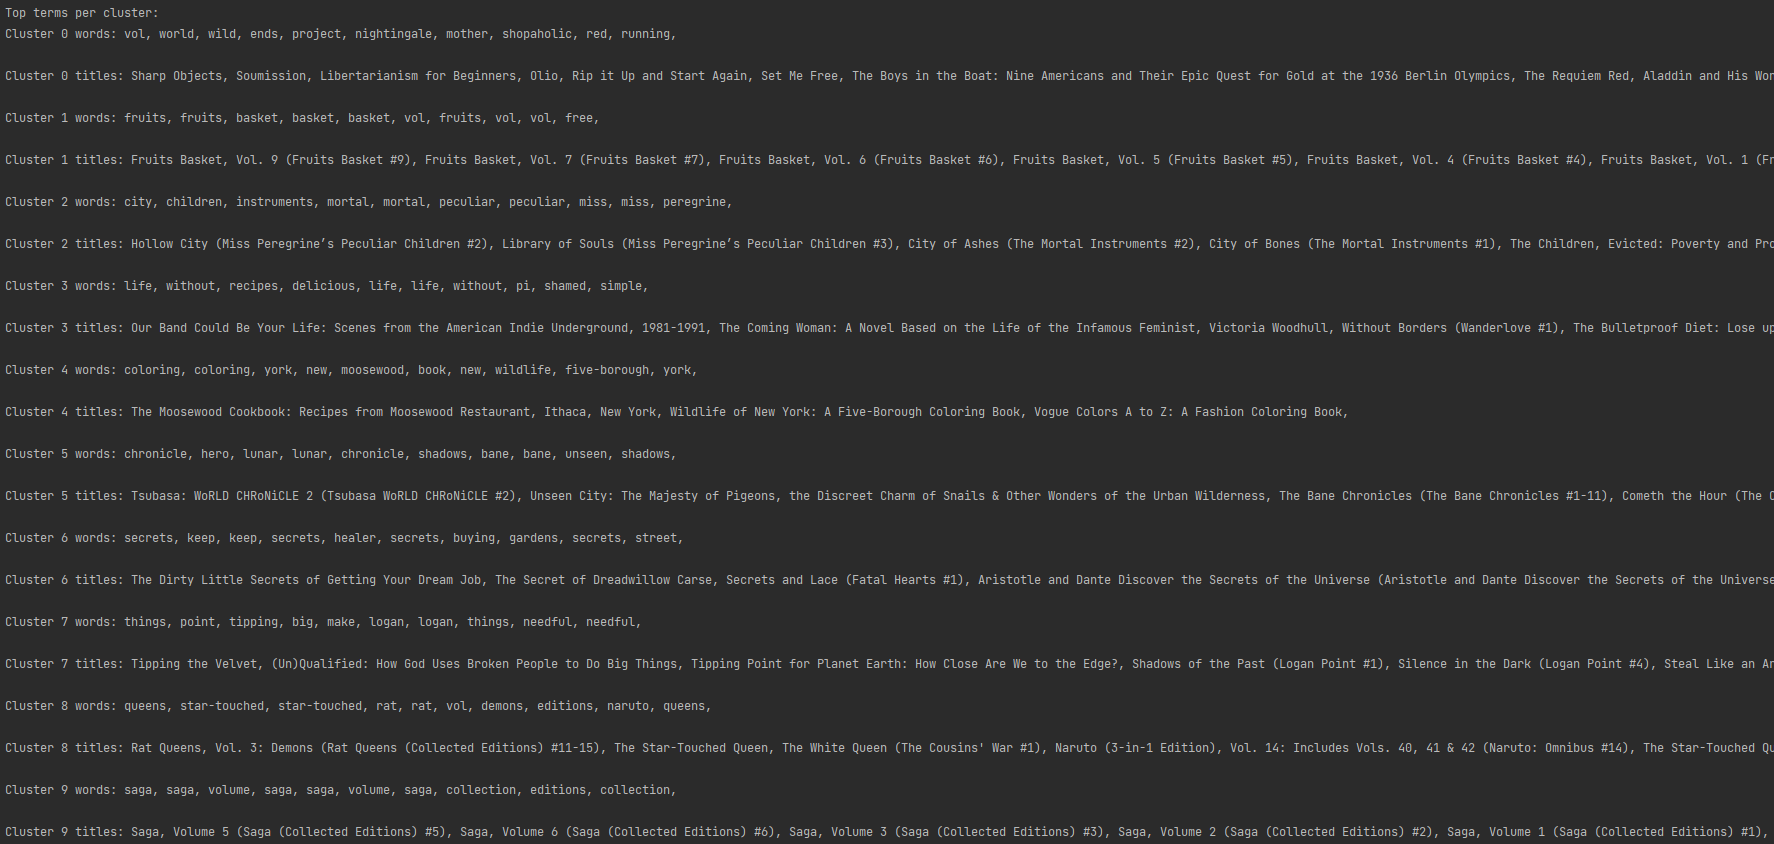
\includegraphics[scale=0.35]{images/results}
	\caption{Resultados del proceso de \textit{clustering}.}
	\label{results}
\end{figure}

\subsection{Evaluación}

En esta sección se intentan evaluar los resultados del proceso de clustering de la sección anterior. Decimos que se intentan evaluar, ya que normalmente la evaluación de un algoritmo de aprendizaje no supervisado es un poco difícil y requiere de ojo humano, que en mi caso no está del todo bien entrenado.

A pesar de ello, con el uso de la librería scikit-learn es usual utilizar dos tipos de métricas para la evaluación de los algoritmos de clustering. Estas dos métricas son: la métrica \textit{homogeneity\_score} y la métrica \textit{silhouette\_score}. En el caso de la práctica usamos la métrica \href{https://scikit-learn.org/stable/modules/generated/sklearn.metrics.silhouette_score.html}{\textit{silhouette\_score}}, que calcula el coeficiente de \href{https://es.wikipedia.org/wiki/Silhouette_(clustering)}{Silhouette}.

El coeficiente de Silhouette toma valores entre -1 y 1. El mejor valor del coeficiente de Silhouette es 1 y el peor valor es -1. Los valores cercanos a 0 nos indicará de la presencia de clústeres superpuestos. Los valores negativos generalmente indican que se han asignado bastantes clústeres de manera incorrecta. Vemos que valor toma a continuación:

\begin{lstlisting}[language=python, basicstyle=\small]
silhouette_coefficient = silhouette_score(tfidf_matrix, labels=kmeans.predict(tfidf_matrix))
print(silhouette_coefficient)
>> 0.024864817391747306
\end{lstlisting}

Entonces, el valor del coeficiente de Silhouette nos indica que los clústeres resultantes de la ejecución de K-Means se superponen. Quizás el ajuste de diferentes parámetros para la extracción de características y el uso de otro algoritmo de clustering aumente esta puntuación.

\section{Conclusiones}

En esta práctica se mostró cómo rastrear contenido de Internet y como agruparlo utilizando el algoritmo K-Means. Hemos podido observar que el algoritmo K-Means puede agrupar textos y que ha agrupado correctamente los títulos de los libros por las palabras que contienen (ver Figura~\ref{results}). Si bien la evaluación de los algoritmos de agrupación en clústeres no es tan fácil en comparación con los algoritmos de aprendizaje supervisado, es deseable tener una idea del rendimiento del algoritmo con anterioridad. Sin embargo, es importante saber qué están midiendo las métricas y si están sesgadas o tienen alguna limitación. 

Puede que el algoritmo elegido no sea el más adecuado para el conjunto de datos de entrada obtenidos por el rastreador, ya que cuando el grupo de datos es grande no hemos conseguido resultados de nuestro agrado, la agrupación ha sido satisfactoria pero hemos obtenido mucho \textit{overlapping} entre los clústeres. Uno de los principales motivos por el que no se ha podido representar los clústeres gráficamente. Seguramente para que el clustering sea más efectivo sería recomendable reducir al mínimo el número de atributos, usar atributos relevantes y poner los datos en una escala similar.

Personalmente mi valoración personal en esta práctica es que me ha parecido muy interesante poder implementar en Python un rastreador web. No lo había hecho nunca y he podido observar con que facilidad y rapidez se puede realizar con el uso de la librería Scrapy. También me ha parecido muy interesante el desarrollo en Python del algoritmo K-Means. Estoy más familiarizada con el desarrollo de modelos de aprendizaje no supervisado en R, y poderlo hacer por primera vez en Python con la librería scikit-learn ha sido muy constructivo. Seguramente ampliaré el uso de esta librería en mis futuros proyectos.

\renewcommand{\refname}{Bibliografía}
\bibliographystyle{unsrt}
\bibliography{biblio}

\end{document}
